\hypertarget{pyinfomap}{\section{Infomap implementation in
Python}\label{pyinfomap}}

\protect\hyperlink{pyinfomap}{}

The code I am submitting is my work on a Python implementation of
Infomap: \url{https://github.com/h1-the-swan/pyinfomap}

As far as I know, there does not yet exist a pure Python implementation
of Infomap, the algorithm to detect communities in network data by
minimizing the map equation. The Infomap software, available at
\url{http://www.mapequation.org/code.html}, is written in C++, although
it has extensions in other languages including Python. A Python
repository was created by Daniel Halperin in 2013.\footnote{\url{https://github.com/uwescience/pyinfomap}}
This code, deemed version 1 by Dr.~Halperin, is capable of calculating
the map equation for a given network and a given two-level clustering of
its nodes.\footnote{By ``two-level clustering'', I mean a
  non-hierarchical, non-overlapping partitioning of each node into
  exactly one of any number of clusters.} My code is a fork of this
repository: I coded the algorithm starting with this base code that can
calculate the function to optimize.

The map equation is (see section
\protect\hyperlink{the-dynamical-perspective}{``The dynamical
perspective''} for background):
\[L(\mathsf{M}) = q_{\curvearrowright} H(\mathcal{Q}) + \sum_{i=1}^{m}{p_{\circlearrowright}^{i} H(\mathcal{P}^i)}\]
where \(\mathsf{M}\) is the module partitioning; the left term is the
average length of codewords (entropy) in the index codebook weighted by
the rate of use of the index codebook \(q_{\curvearrowright}\); and the
right term is the average length of codewords in module codebook \(i\)
weighted by the rate of use of this module \(p_{\circlearrowright}\).
Using \(q_{\curvearrowright} = \sum_{i=1}^{m}{q_{i\curvearrowright}}\);
\(p_{\circlearrowright}^{i} = \sum_{\alpha \in i}{p_{\alpha}} + q_{i\curvearrowright}\)
where \(\alpha \in i\) means every node in module \(i\) (the
\(q_{i\curvearrowright}\) is added as the probability that the random
walker exits the module and the exit codeword is used); and the
definition of entropy\footnote{For a random variable \(X\) that can have
  \(n\) states with probability \(p_i\), the entropy is
  \(H(X) = -\sum_{i=1}^{n}{p_i\log{p_i}}\).}, the map equation can be
expanded to: \[
\begin{aligned}
L(\mathsf{M}) = &\left(\sum_{i=1}^{m}{q_{\curvearrowright}}\right) 
                                        \log \left(\sum_{i=1}^{m}{q_{\curvearrowright}}\right)
                                        - 2 \sum_{i=1}^{m}{q_{\curvearrowright}} \log (q_{\curvearrowright)} \\
                                &- \sum_{\alpha=1}^{n}{p_{\alpha} \log(p_\alpha)}
                                        + \sum_{i=1}^{m}{\left(q_{\curvearrowright} + \sum_{\alpha \in i}{p_{\alpha}}\right) \log \left(q_{\curvearrowright} + \sum_{\alpha \in i}{p_{\alpha}}\right)}
\end{aligned}
\]

The node visit probability \(p_{\alpha}\) is related to the dynamics
being modeled. Dr.~Halperin's code uses PageRank with teleportation
probability \(\tau = 0.15\). This is modeling a random walker on the
network that has a 15\% chance, on every step, of teleporting to a
random node instead of following a link as normal. The code uses the
Python package NetworkX \TODO{cite} to handle graph storage and
operations; this package has its own method for calculating PageRank for
every node. The exit probability \(q_{i\curvearrowright}\) is then
calculated as \autocite{rosvall_map_2010}:
\[q_{i\curvearrowright} = \tau \frac{n-n_i}{n} \sum_{\alpha \in i}{p_{\alpha}} + (1-\tau) \sum_{\alpha \in i}{\sum_{\beta \notin i}{p_{\alpha}w_{\alpha \beta}}}\]
where \(n_i\) is the number of nodes in module \(i\), and
\(w_{\alpha \beta}\) is the normalized weight of the link from
\(\alpha\) to \(\beta\) (if \(\alpha\) is a dangling node, this weight
is replaced by \(1-n_i/n\)).

Version 1 implements a \texttt{Module} class and a \texttt{Clustering}
class. I build a \texttt{PyInfomap} on top of these in order to be able
to calculate the map equation for different clusterings of an input
graph. What follows is my work implementing an optimization algorithm.

The test example I use is network (a) in Fig.~\ref{fig:mapvsmod} in this
document (Fig. 3 in \autocite{rosvall_map_2010}). A pajek version of
this network was included in the forked repository as
\texttt{2009\_figure3ab.net}. We know that the clustering seen in the
figure should have a value for the map equation \(L = 3.33\). We know
from the text that the clustering seen in the figure should have a value
for the map equation \(L = 3.33\), and that this is the optimal
(minimum) value for this network. Thus, my algorithm should be able to
find this clustering.

One approach to find the clustering would be to calculate the map
equation for every possible partition of the network. I implement this
in \texttt{search\_all\_possible\_partitions.py}. However, there are far
too many combinations of partitions for network data, even for the small
16-node network I use to test. As of this writing, this code has not yet
finished after running for 212 hours (almost 9 days), having tried over
\(6.15 \times 10^9\) different partitions.

A more realistic option is to use some sort of search algorithm. I
implement the Louvain method, which was originally developed as a
modularity-optimizing community detection algorithm
\autocite{blondel_fast_2008}, and which is the starting point for the
official version of Infomap \autocite{rosvall_map_2010}. This method
consists of two phases, which are performed repeatedly. It starts with
every node in it's own separate module. In the first phase, each node,
one at a time in random order, is moved to be in the same module as its
neighbor that gives the lowest value of the map equation. This is
repeated until no improvement can be made. In the second phase, a new
network is constructed in which the nodes represent the clusters found
in the previous step, edges are weighted by the number of
between-cluster edges in the original graph, and within cluster edges
become self-loops (i.e., edges from one node in the new network to
itself). The algorithm is then repeated on this new graph, with each
calculation of the map equation done using the original graph. Phase one
and two are repeated until no improvement is seen.
Fig.~\ref{fig:louvain} shows a schematic of this procedure.

\begin{figure}
\centering
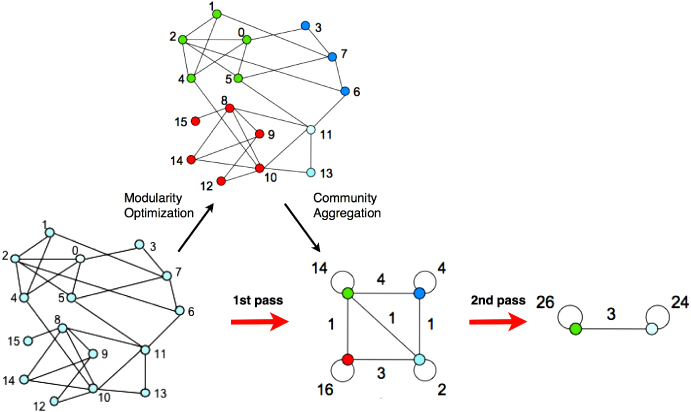
\includegraphics{img/blondel2008_fig1_louvain.jpg}
\caption{Schematic of the Louvain algorithm from
\autocite{blondel_fast_2008}. Each pass consists of a phase in which
local merges of communities are made to optimize the objective function,
and a phase in which a new meta-graph is constructed with the
communities as nodes. The two phases are repeated until no improvement
is found.}\label{fig:louvain}
\end{figure}

The official Infomap algorithm takes additional steps after this point
to broaden the search space and avoid local optima. These include
recursively running the algorithm on the clusters, and freeing
individual nodes to move between modules. My implementation does not yet
include this.

My implementation can find the optimal four-way partition of the test
network. It can also find the optimal partition for network (d) in the
same figure, in which all nodes are grouped into the same module. It run
in under 1 second on these test networks (after loading the needed
libraries). It is able to run the larger karate club network (34 nodes)
in under 5 seconds.

Next steps would include tests on synthetic benchmarks, and further
analysis of the results of the karate club network, as well as other
standard examples (see section
\protect\hyperlink{evaluation}{``Evaluation of community detection
methods''}).
